\subsection{Delta Functions}
\subsubsection{Discrete Functions}
So far we have seen functions expressed in the continuous domain of real numbers. $f(x),\ x\in\R$ but we can change the domain of our function to, say, complex numbers or integers. A function that can only take in integer values of $x$ is called a discrete (or discrete-time) function and will usually be expressed in the form $x[n]$.\\
Discrete functions will work similarly to their continuous counterparts for many applications but with some caveats. One of the major differences is that an expression such as $x[\frac{1}{2}]$ is undefined as it can not take in a non-integer input.\\
This means that there is a larger branch of functions that will not have an inverse.\\
For example, if we have some function $x[n]$, we can scale it to get $y[n]=x[2n]$, however, if we then want to go back, we cannot get back $x[n]$ from $y[n]$ as it would require us to take $x[n]=y[\frac{n}{2}]$ which is undefined for odd $n$.\\
Another notion that we have in continuous time that we don't have in discrete time is derivatives. What we have instead is finite differences. If you recall, a derivative is simply the limit of the change in $y$ over the change in $x$ ($\frac{\Delta y}{\Delta x}$) as $\Delta x\to0$. Because discrete functions can only take in integer values, this limit will not exist and we are instead left with a finite difference equation such as $y[n]=x[n]+x[n-1]$.\\

We can solve difference equations in a few ways similar to how we might solve differential equations.\\
One way is the method of recursion. If we assume that our system turns on at $n=0$ we can state that $y[-1]=0$ and solve our difference equation recursively. Note that this can be a realistic assumption as we may wish to find the recursive form of the coefficients of a series we know starts at $n=0$.\\
Ex: $y[n]-ay[n-1]=K\delta[n]$
\begin{align*}
    &y[n]=ay[n-1]+K\delta[n]\\
    &n=0:\ y[0]=ay[-1]+K=K\\
    &n=1:\ y[1]=ay[0]=aK\\
    &n=2:\ y[2]=ay[1]=a^2K\\
    &n=3:\ y[3]=ay[2]=a^3K\\
    &\Ra y[n]=a^nK
\end{align*}

\subsubsection{Kronecker Delta Function}
Now that we have seen some more complicated Power series examples, let's take a moment to go back to one of the simplest power series: $f(x)=x$. Using the general form of the Power series centered about $x=0$ we have
$$f(x)=\sum_{n=0}^\infty A_nx^n$$
Setting $f(x)=x$ we will only have the $n=1$ term of the series. If we want to express this with our series notation, it corresponds to an $A_n$ that satisfies
$$A_n=\eqnsystem{1, & n=1\\ 0, & n\neq 1}$$
Turns out that being able to generalize this coefficient in the series is somewhat useful as you may want to work with expressions in terms of series to add terms or get your expression in a familiar form. Our current expression is represented as a piecewise function which is not the nicest to work with. This is a common enough expression, however, that it is well defined.\\
We can express the Kronecker delta function as a discrete function that attains a value of 1 when $n=i$ and is 0 everywhere else
$$\boxed{\delta_{ni}=\eqnsystem{1, & n=i\\ 0, & n\neq i}}$$
This may also be written as a discrete-time function
$$\delta[n-i]=\delta_{ni}=\eqnsystem{1, & n=i\\ 0, & n\neq i}$$
At some points it may be easier to represent the Kronecker delta function using one notation vs. another but they mean the same thing. For this chapter, we will primarily use the discrete-time notation whereas in PDEs you will likely see this using the subscript notation.\\

We can express any series as a weighted sum of Kronecker delta functions:
$$A_n=\sum_{k=-\infty}^\infty A_k\delta[n-k]$$
where $A_n$ represents the coefficients inside a summation.\\
To generalize this further, instead of looking at coefficients inside a series, let's look at a function in discrete-time, $x[n]$.
$$x[n]=\sum_{k=-\infty}^\infty x[k]\delta[n-k]$$
So by applying some operation involving the delta function and the function $x[n]$, we get back the same function $x[n]$. This operation is called the discrete-time convolution and is defined as follows:
$$\boxed{x[n]*y[n]=\sum_{k=-\infty}^\infty x[k]y[k-n]}$$
Note that it doesn't matter which order you convolve the functions in:
$$x[n]*y[n]=y[n]*x[n]$$
$$\sum_{k=-\infty}^\infty x[k]y[k-n]=\sum_{k=-\infty}^\infty y[k]x[k-n]$$
The delta function happens to be the identity function for this operation. This means that any function convolved with the delta function will give back the original function.\\
Convolution of two functions corresponds to taking one function and ``sweeping" it over another function, multiplying the overlapping terms and summing them. So places where the functions overlap more will have their convolution be more positive.\\
\centerline{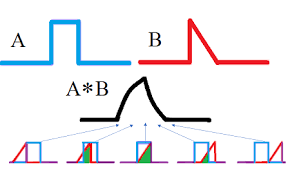
\includegraphics[scale = 0.8]{Images/FourierImages/Convolution.png}}

\subsubsection{Dirac Delta Function}
Convolution is not limited to discrete functions. Keeping with the idea of sweeping a function over another one and recording a value for each time step can be achieved for continuous functions as well. The main difference is that the convolution must also be continuous as we need to record a value for each time step for all real numbers.\\
We can express the convolution using integrals instead of sums in order to achieve this:
$$\boxed{f(x)*g(x)=\int_{-\infty}^\infty f(\tau)g(t-\tau)d\tau}$$
The convolution in continuous-time will have the same commutative property as that in discrete-time.\\
We can also aim to find a similar identity function for continuous-time convolution.
\begin{align*}
    &f(t)=f(t)*\delta(t)=\int_{-\infty}^\infty f(\tau)\delta(t-\tau)d\tau
\end{align*}
Because we want to express the result of our integral as $f(t)$ we can say that we will only get a $f(t)$ term for where $\tau=t$. This corresponds to
\begin{align*}
    &\delta(x)=\eqnsystem{\delta(0) & x=0\\ 0 & x\neq 0}
\end{align*}
This looks similar to the delta function in the discrete case (as you may have guessed) but with the slight difference in that the continuous case has a singularity. To find the value of this singularity, let's look at the case $f(t)=1$.
\begin{align*}
    &1=\delta(t)*1=\int_{-\infty}^\infty\delta(\tau)d\tau
\end{align*}
This is a defining property of the delta function in continuous time and allows us to properly define what we call the \textit{Dirac delta function}:
$$\boxed{\delta(x)=\eqnsystem{\infty & x=0\\ 0 & x\neq 0},\quad\quad \int_{-\infty}^\infty \delta(x)dx=1}$$
There are many ways to express this analytically but the most intuitive way may be to imagine the Dirac delta function as an infinitely tall rectangle with an area of 1.\\
The Dirac delta function will also give the property
$$\boxed{f(a)=\int_{-\infty}^\infty f(x)\delta(x-a)dx}$$
which allows us to express the Dirac delta function as the identity function in the continuous-time convolution operation.
Some other properties of the Dirac delta function are as follows:
$$\delta(x)=\delta(-x)$$
$$\delta(ax)=\frac{1}{|a|}\delta(x)$$
$$\delta(x^2-a^2)=\frac{1}{|2a|}\brround{\delta(x-a)+\delta(x+a)}$$
$$\delta((x-a)(x-b))=\frac{1}{|a-b|}\brround{\delta(x-a)+\delta(x-b)}$$

\subsubsection{Step Function}
We can introduce another function called the unit step (or Heaviside) function. This is defined as
$$\boxed{u(t)=\eqnsystem{1 & x>0\\ 0 & x<0}}$$
If we shift the function, we get $u(t-a)$ or $u_a(t)$ which means that the function jumps to the value 1 at time $a$ instead of time 0.\\
This function is particularly useful in expressing piecewise functions. For example, if we have the function
\begin{align*}
    &f(x)=\eqnsystem{x & x>0\\ 0 & x<0}
\end{align*}
Then we can express it using the unit step as one function
\begin{align*}
    &f(x)=xu(x)
\end{align*}
Ex2:
\begin{align*}
    &f(x)=\eqnsystem{1 & x<0\\ \cos x & 0\leq x< \pi\\ -1 & x\geq \pi}
\end{align*}
We can rewrite this as
\begin{align*}
    &f(x)=u(-x)+\cos(x)u(x)-\cos(x)u(x-\pi)-u(x-\pi)\\
    &f(x)=u(-x)+\cos(x)u(x)-(1+\cos(x))u(x-\pi)
\end{align*}
The unit step isn't necessarily defined at 0, however, a common convention would be to set $u(0)=\frac{1}{2}$. This allows for the following property to become true everywhere
$$u(x)+u(-x)=1$$
Another defining property of the unit step function is its derivative. Because it's not a continuous function, it doesn't have a derivative but let's ignore that for a moment. Let us define the unit step as follows:
\begin{align*}
    &u(x)=\lim_{\epsilon\to0}\eqnsystem{0 & x<-\epsilon\\ \frac{x}{2\epsilon} & -\epsilon<x<\epsilon\\ 1 & x>\epsilon}
\end{align*}
This expression of the unit step in the limit makes it continuous so let's take the derivative:
\begin{align*}
    &\ddx{x}u(x)=\lim_{\epsilon\to0}\eqnsystem{0 & x<-\epsilon\\ \frac{1}{2\epsilon} & -\epsilon< x<\epsilon\\ 0 & x>\epsilon}
\end{align*}
In the limit we have the derivative is equal to infinity at 0 and 0 everywhere else. If we take the integral, we'll see that this function has an area of 1.
\begin{align*}
    &\int_{-\infty}^\infty\ddx{x}u(x)dx=\lim_{\epsilon\to0}\int_{-\epsilon}^\epsilon\frac{dx}{2\epsilon}=1
\end{align*}
These two properties imply that the derivative of the unit step is the Dirac delta function
$$\boxed{\ddx{x}u(x)=\delta(x)}$$
The step function is defined similarly for discrete-time as well
$$\boxed{u[n]=\eqnsystem{1 & n\geq 0\\ 0 & n<0}}$$
We can also relate this to the Kronecker delta function through a difference equation:
$$\boxed{u[n]-u[n-1]=\delta[n]}$$

\subsubsection{Calculus of Piecewise Functions}
When we go to integrate the step function, we can take advantage of the property that it is zero for half of its domain and change the bounds of the integral:\\
Ex:
\begin{align*}
    &\int_{-5}^5 u(x)dx=\int_0^5 1dx=5
\end{align*}
This greatly simplifies integrals involving a step function. If you recall from the fundamental theorem of calculus, we can define a function as
$$F(x)=\int_0^x f(t)dt+F(0)$$
With most functions, taking this integral is no issue (aside from maybe changing the domain to where the function is defined). For a piecewise function, however, we need to be careful about how we treat the $x$ in the integral as the function will change how it's described depending on the value of $x$.\\
Ex:
\begin{align*}
    &\int_1^x\delta(t)dt
\end{align*}
The function changes values at $x=0$ so we will want to look at two cases:
Case $x>0$:
\begin{align*}
    &\int_1^x\delta(t)dt=0
\end{align*}
Case $x<0$:
\begin{align*}
    &\int_1^x\delta(t)dt=-\int_x^1\delta(t)dt=-1
\end{align*}
This means that our solution will be a piecewise function as well
\begin{align*}
    &\int_1^x\delta(t)dt=\eqnsystem{0 & x>0\\ -1& x<0}
\end{align*}
We can define this using the step function
\begin{align*}
    &\int_1^x\delta(t)dt=-u(-x)
\end{align*}
Interestingly, this integral can be generalized depending on the value of the lower bound of the integral as it will impact which of the above two cases gives a nonzero result.
$$\int_a^x\delta(x)dt=\eqnsystem{u(x) & a<0\\ -u(-x) & a>0}$$
If we multiply by a function in the integral, this turns into
$$\int_a^xf(t)\delta(t)dt=\eqnsystem{f(0)u(x) & a<0\\ -f(0)u(-x) & a>0}$$
For the step function we can do similar:\\
Ex:
\begin{align*}
    &\int_{-1}^xu(t)dt
\end{align*}
Case $x>0$:
\begin{align*}
    &\int_{-1}^xu(t)dt=\int_0^x1dt=x
\end{align*}
Case $x<0$:
\begin{align*}
    &\int_{-1}^xu(t)dt=0\\
    &\int_{-1}^xu(t)dt=\eqnsystem{x & x>0\\ 0 & x<0}\\
    &\int_{-1}^xu(t)dt=xu(t)
\end{align*}
Ex2:
\begin{align*}
    &\int_1^xu(t)dt
\end{align*}
Case $x>0$:
\begin{align*}
    &\int_1^x 1dt=x-1
\end{align*}
Case $x<0$:
\begin{align*}
    &\int_1^x u(t)dt=0\\
    &\int_1^xu(t)dt=(x-1)u(t)
\end{align*}
We can come up with general equations for the integral of a step function as
$$\int_a^x u(t)dt=(x-a)u(x)$$
$$\int_a^x u(-t)dt=(x-a)u(-x)$$
If we take the integral of a function times the step function, we get
$$\int_a^xf(t)u(t)dt=\eqnsystem{\ds\int_a^xf(t)dtu(x) & a>0\\ \ds\int_0^xf(t)dtu(x) & a\leq0}$$
Derivatives will work similarly to regular calculus.\\
Ex:
\begin{align*}
    &\ddx{x}f(x)u(x)=f'(x)u(x)+f(x)\delta(x)
\end{align*}
This corresponds to the regular derivative plus the impulse that comes from the jump discontinuity of the step function.\\
Also note that because the delta function is only nonzero in one place we can express a function times the delta function as
$$f(x)\delta(x-a)=f(a)\delta(x-a)$$

\subsubsection{Common Piecewise Functions and Binary Logic}
We have already seen some previous examples of operations that create piecewise functions.\\
One of the most common ones may be the absolute value of a function and can be rewritten as
$$|x|=x(u(x)-u(-x))$$
The absolute value of a general function is not as intuitive to express using piecewise functions and so it is better to leave absolute value functions as they are as they already compress a piecewise function. It can be helpful to use absolute value statements in conjunction with step functions in order to make statements more compact.\\
Another example we've seen is the sign function which returns whether a number is positive or negative.
$$\sgn(x)=\eqnsystem{1 & x>0\\ -1 & x<0}$$
This can be rewritten using the step function as
$$\sgn(x)=2u(x)-1$$
Another function that is less talked about but is widely used in some applications is the ramp (or ReLU) function defined as
$$\mathrm{ramp}(x)=\eqnsystem{x & x>0\\ 0 & x\leq 0}=\max\brcurly{0,x}=xu(x)$$
The max operator is another tool we can use to express piecewise functions.\\
One significant advantage that the step function offers us is that it has a well known derivative. The derivative of the max operator is not defined like it is for the step function. The derivative of the absolute value operation is loosely defined as the sign function, however, it takes a little more work to manipulate expressions using the sign function than it does the step function.
\begin{align*}
    &\ddx{x}|x|=\ddx{x}\brround{x(u(x)-u(-x))}\\
    &=u(x)-u(-x)+x\brround{\delta(x)+\delta(-x)}\\
    &\text{using }f(x)\delta(x)=f(0)\delta(x)\text{ and }\delta(x)=\delta(-x)\\
    &\ddx{x}|x|=u(x)-u(-x)+(0)(2\delta(x))\\
    &=u(x)-u(-x)+1-1\\
    &=u(x)-u(-x)+u(x)+u(-x)-1\\
    &=2u(x)-1\\
    &=\sgn(x)
\end{align*}
Another common expression is a square or rectangular pulse. We can represent this as
$$f(x)=u(x)-u(x-1)$$
This is the standard way of representing a constant pulse. This means for every pulse we'll have to use two step functions. If we wish to represent a rectangle wave (repeated periodic rectangular pulses) this would take infinitely many step functions. We can, however, express it more elegantly as the step function of a periodic function
$$\mathrm{rect}(x)=u(\sin(x))$$
or as
$$\mathrm{rect}(x)=\sgn(\sin(x))$$
Note that these two functions will not be equal as they differ by a vertical shift but they achieve the same goal of a having a periodic rectangular pulse.\\

The idea of being able to turn a function on and off depending on its sign lends itself well to binary operations and logic gates. We can take some random function $x(t)$ and by taking the step response of the function, we can output a response, $f(t)$, that is only turned on when the function is positive.
\[ f(t)=u(x(t)) \]
We can determine the NOT operator to be when the function is negative
\[ f(t)=u(-x(t)) \]
We can mix two functions together to get the standard logic gates which, once those are expressed, can be used to form any binary computation in the way that computers work.\\
An XOR gate can be achieved as
$$f(t)=u(x(t)y(t))$$
An AND gate can be achieved as
$$f(t)=u(x(t))u(y(t))$$
From these, we can easily get the opposite gates such as NAND or NXOR by doing
$$f_\text{NOT}(t)=1-f(t)$$
The above expressions are the easiest ones to express and have a natural way of being written. The other expressions are less obvious and can be expressed in many different possible ways, including using the other gates. Here is an example of how they can be expressed:\\
For an OR gate:
$$f(t)=u\brround{u(x(t))+u(y(t))-\frac{1}{2}}$$